\documentclass{article}
\title{The Mind, Spring 2013\\ Lab \#4: Acoustic Measurements}
\author{Instructor: Diogo Almeida}
\usepackage{booktabs}
\usepackage{graphicx}
\usepackage{apacite}
\usepackage{paralist}
\usepackage{tipa}
\usepackage[colorlinks]{hyperref}
\hypersetup{%
	pdftitle={Lab 4 - The Mind - Acoustic Measurements},
	pdfauthor={Diogo Almeida},
	pdfkeywords={acoustics, acoustic phonetics, vowel, formants, VOT, formant transitions, consonants, acoustic correlates, segments, NYUAD, The Mind, tutorial},
	breaklinks,
	bookmarksnumbered,
	bookmarksopen,
	pdfpagemode=UseOutlines,
	pdfstartview={FitH},
	urlcolor=cyan,
	linkcolor=blue,
}%

\newcommand{\soft}[1]{\textsf{#1}}
\newcommand{\filefmat}[1]{\texttt{#1}}
\newcommand{\printurl}[1]{\texttt{#1}}
\newcommand{\softmenu}[1]{\texttt{#1}}
\newcommand{\doscommand}[1]{\texttt{#1}}

\newcommand{\MSExcel}{\soft{Microsoft\texttrademark{} Excel}} 
\newcommand{\OpOff}{\soft{LibreOffice}}
\newcommand{\Praat}{\soft{Praat}}
\newcommand{\tform}{\soft{TreeForm}}
\newcommand{\Classes}{\soft{Classes}}

\begin{document}
\maketitle

\tableofcontents
\newpage
\listoffigures
\newpage
\section{Overview}

This is the fourth lab of the semester. It is divided into three parts. In the first one, you will be measuring the values of the formants for English vowels. In the second one, you will be trying to find acoustic correlates of stop consonants in English. In the third and final part, you will be measuring acoustic information responsible for making the difference between voiced and unvoiced stop consonants (for instance, between [b] and [p].

In order to accomplish this, you will be making your own recordings and analyzing your own utterances. You'll be using \Praat{} for these tasks. \Praat{} is a free, cross--platform, open--source phonetic analysis package that can be downloaded from \href{http://www.praat.org}{http://www.praat.org}.

\section{Part 1: Vowel Formant Analysis}

In this part, you will analyze recordings of a native speaker of American English uttering the following words:

\begin{enumerate}
\item heed -- [h i\textlengthmark{} d]
\item hid -- [h \textsci{} d]
\item head -- [h \textepsilon{} d] 
\item had -- [h \ae {} d]
\item hod -- [h \textscripta\textlengthmark{} d]
\item hawed -- [h \textopeno\textlengthmark{} d]
\item hood -- [h \textupsilon{} d]
\item who'd -- [h u\textlengthmark{} d]
\end{enumerate}

The speaker repeated each word 5 times. Your goal is to open these different files, then get the vowel formants (F1, F2 and F3) values as given by \Praat{} and store them in a spreadsheet program --- \MSExcel{} or \OpOff{} are fine. Remember to label each column and line so you know what the values refer to.

Once you have measured all the formant values of your recordings, you should average the values of the formants for each vowel and then plot those in a F1-F2 graph (F1 as the y--axis and F2 as the x--axis).

\subsection{Open file and look at the spectrogram}

Open \Praat{}. You will see two windows: \softmenu{Praat Objects} and \softmenu{Praat Picture}. Go to the \softmenu{Praat Objects} window, and click  \softmenu{Open} $>$ \softmenu{Read from file\ldots}), and select one of the sound files in the folder you just downloaded from \Classes{}.

Once you see the file in the \softmenu{Objects} list (figure~\ref{step1look}), go to the spectrogram view (\softmenu{View \& Edit}, see figure~\ref{step2look}).

\begin{figure}[!tbp]
\caption{\Praat{} -- Object in List}
\label{step1look}
	\begin{center}
		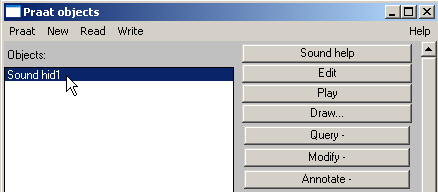
\includegraphics[width=0.8\textwidth]{PraatObjectinList}
	\end{center}
\end{figure}

\begin{figure}[!tbp]
\caption{\Praat{} -- How to display the Spectrogram}
\label{step2look}
	\begin{center}
		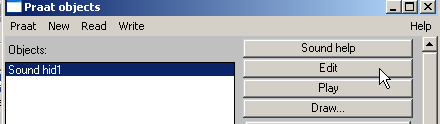
\includegraphics[width=0.8\textwidth]{PraatEditButton}
	\end{center}
\end{figure}

This will open a window where you can see both the waveform and its spectrogram (figure~\ref{step3look}). If you can't see the spectrogram, go to \softmenu{Spectrum} $>$ \softmenu{Show Spectrogram}.

In case your spectrogram is not as clear as the one we saw in class or as the one I show here (figure~\ref{step3look}), you can try to ``prettify'' the spectrogram a little bit. Go to \softmenu{Spectrum} $>$ \softmenu{Spectrogram settings}. Look for the \softmenu{Dynamic Range} (dB) field (figure~\ref{step4look}). The default value is 50 (and for reasons I don't quite understand, sometimes 70). Try lowering it in 3dB decrements and see what it does to your spectrogram. Can you see your formants a little better? Compare figures~\ref{step3look} and~\ref{step5look}.

\begin{figure}[!tbp]
\caption{\Praat{} -- Edit Window}
\label{step3look}
	\begin{center}
		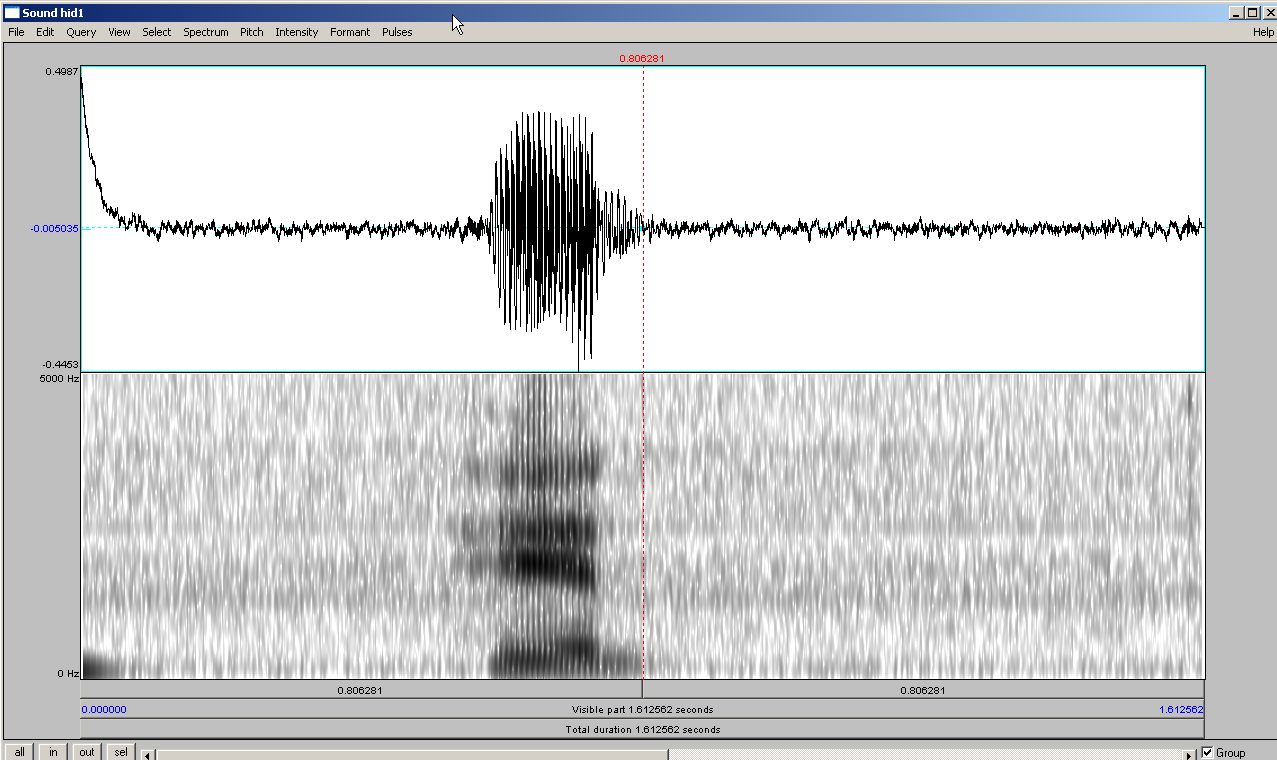
\includegraphics[width=0.8\textwidth]{PraatEditWindow}
	\end{center}
\end{figure}

\begin{figure}[!tbp]
\caption{\Praat{} -- Changing the value of Dynamic Range}
\label{step4look}
	\begin{center}
		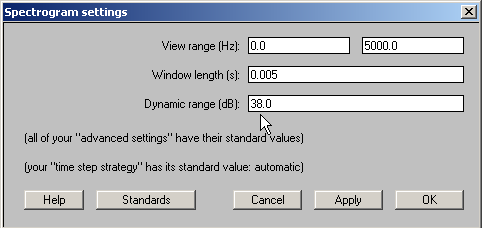
\includegraphics[width=0.8\textwidth]{PraatEditWindowSpectroSettingsDynRange}
	\end{center}
\end{figure}

\begin{figure}[!tbp]
\caption{\Praat{} -- Edit Window with modified Dynamic Range value (38dB)}
\label{step5look}
	\begin{center}
		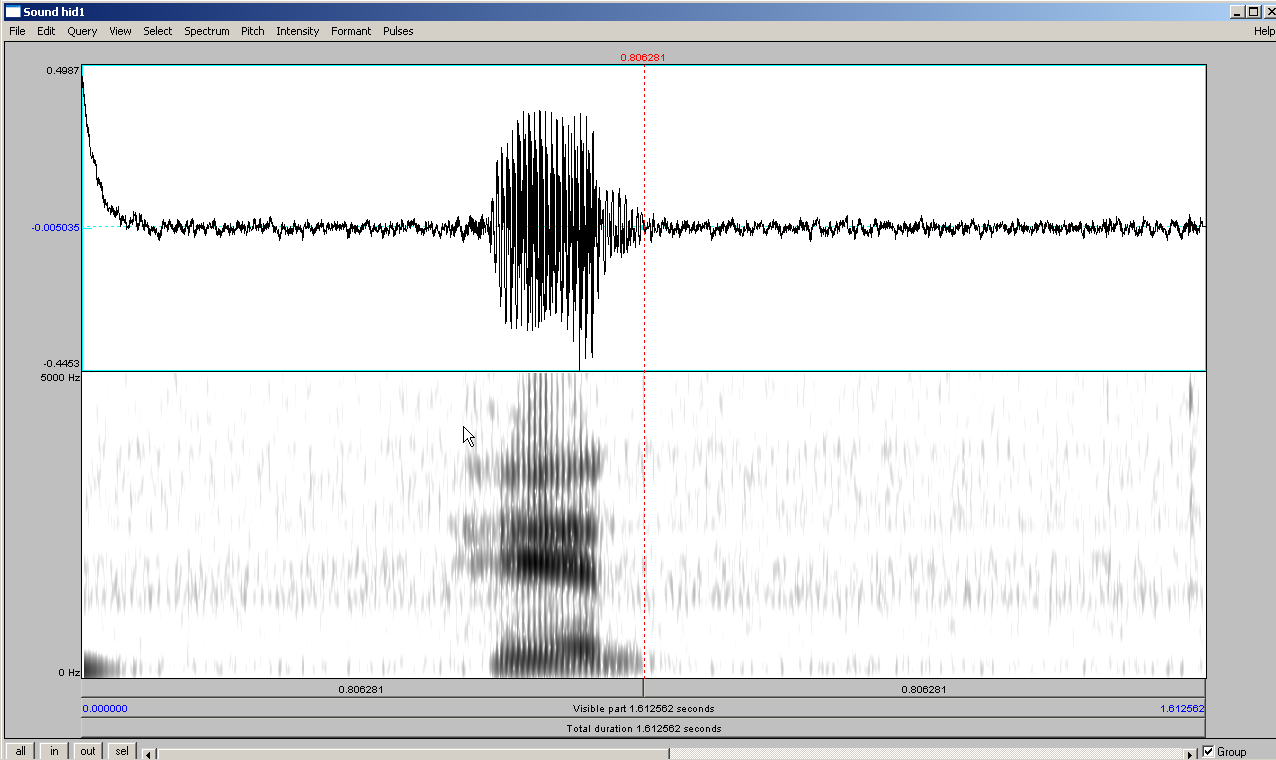
\includegraphics[width=0.8\textwidth]{PraatEditWindowPretty41dB}
	\end{center}
\end{figure}

\subsection{Making the measurements}

Once you have your spectrogram in front of you, go to \softmenu{Formant} $>$ \softmenu{Show Formants}. You should see the formants with a bunch of red dots overlaid (figure~\ref{step1measure})

\begin{figure}[!tbp]
\caption{\Praat{} -- Formant tracking}
\label{step1measure}
	\begin{center}
		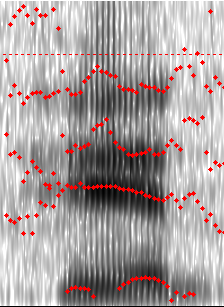
\includegraphics[width=0.8\textwidth]{PraatFormantTrack}
	\end{center}
\end{figure}

As you can see, \Praat{}'s formant tracking algorithm is pretty neat, but it is not flawless. Notice the gap in F1 and the bump in F3 (figure~\ref{step1measure})?

\begin{figure}[!tbp]
\caption{\Praat{} -- Selecting the window of interest for the measurement of the Formants}
\label{step2measure}
	\begin{center}
		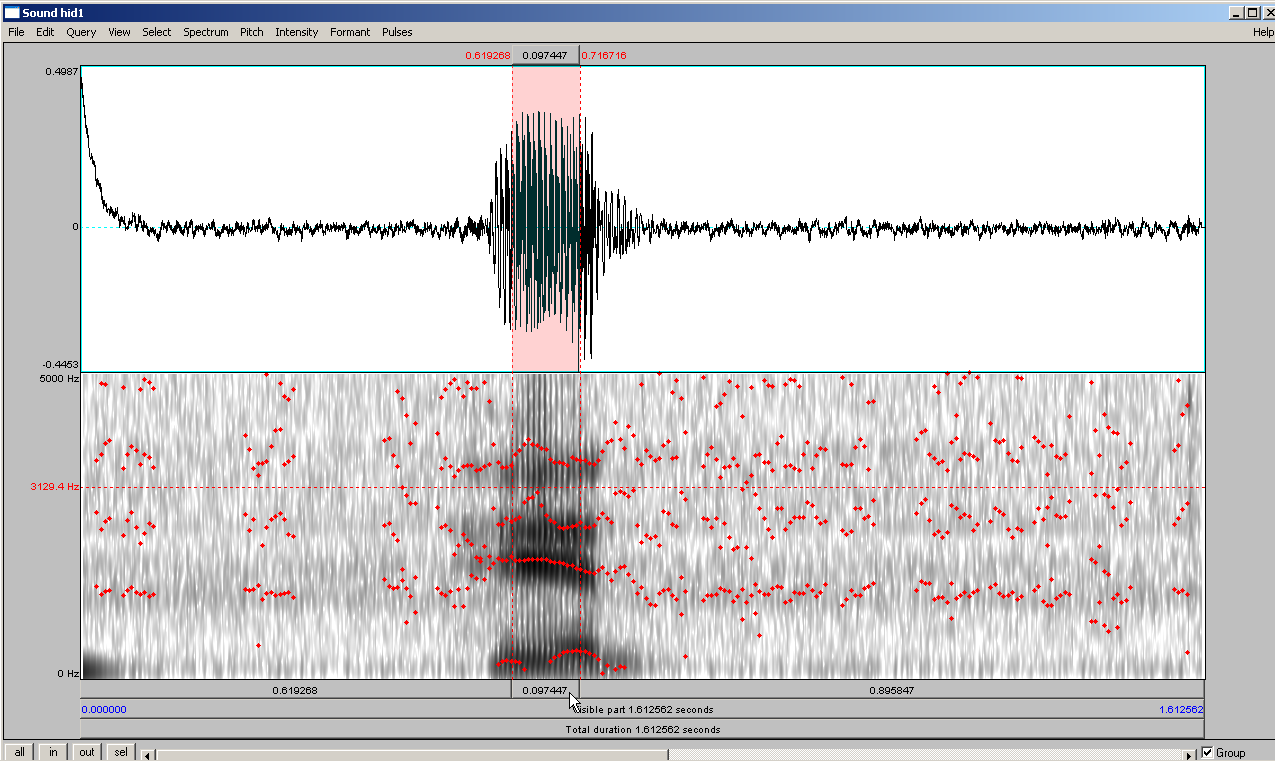
\includegraphics[width=0.8\textwidth]{PraatSpectrogrSelection}
	\end{center}
\end{figure}

If \Praat{} gave you reasonable formant tracks, then you can select a window over the center of the vowel (figure~\ref{step2measure}) --- a tip: to play the selection, click where the mouse cursor is on figure~\ref{step2measure} --- and go to \softmenu{Get first formant} (figure~\ref{step3measure}). This should give you a window with a value. Notice what the value actually is.

\begin{figure}[!tbp]
\caption{\Praat{} -- Getting the Formants automatically}
\label{step3measure}
	\begin{center}
		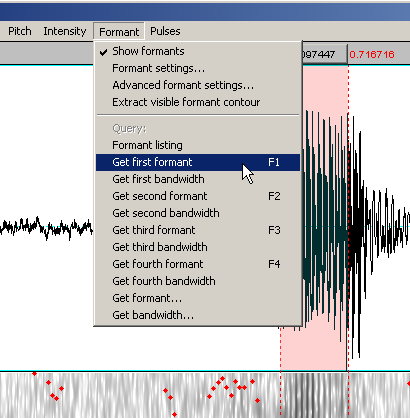
\includegraphics[width=0.8\textwidth]{PraatSpectrogrGetF1}
	\end{center}
\end{figure}


If \Praat{} gave you formant tracks that don't seem to capture the formants you see adequately, then you can try to pin a couple of points in the formants, get their values, average them and record that value in the spreadsheet. To get the value of any particular point, you can just click on it and \Praat{} will give you its value on the left side of the spectrogram (figure~\ref{step4measure}). You can then jot down the numbers somewhere. If you want numbers that you can copy and paste, just click on the point, and then go to \softmenu{Spectrum} $>$ \softmenu{Get frequency at cursor} (figure~\ref{step5measure}).

\begin{figure}[!tbp]
\caption{\Praat{} -- Getting the Formants with the mouse}
\label{step4measure}
	\begin{center}
		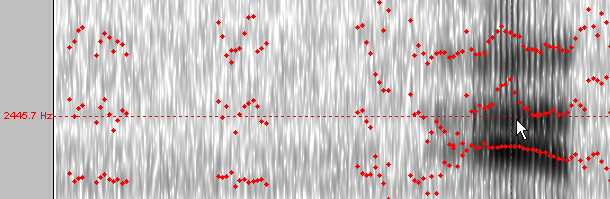
\includegraphics[width=0.8\textwidth]{PraatSpectrogrGetF1byCursor}
	\end{center}
\end{figure}

\begin{figure}[!tbp]
\caption{\Praat{} -- In case you want to copy and paste your pinpointed Formant value}
\label{step5measure}
	\begin{center}
		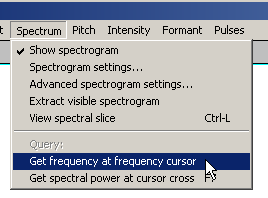
\includegraphics[width=0.8\textwidth]{PraatSpectrogrGetF1byCursorMenu}
	\end{center}
\end{figure}

If you decide to do that, then you should be consistent across measurements. Choose the same number of points and be explicit about why you decided to take them.  

\subsection{Saving and Plotting the Formant values}

\subsubsection{Saving the values}
Once you get your values, you should start saving them into a spreadsheet. Remember to label the values (figure~\ref{step1save}).

\begin{figure}[!tbp]
\caption{\MSExcel{} -- Saving the Formant values of each recording}
\label{step1save}
	\begin{center}
		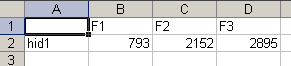
\includegraphics[width=0.8\textwidth]{Excel1}
	\end{center}
\end{figure}

Once you finished copying the values to the spreadsheet, you will have to average them. In figure~\ref{step2save}, you can see that~\MSExcel{} has a function to do the averaging for you.

\begin{figure}[!tbp]
\caption{\MSExcel{} -- Averaging Formant values. \emph{These values are made up}!}
\label{step2save}
	\begin{center}
		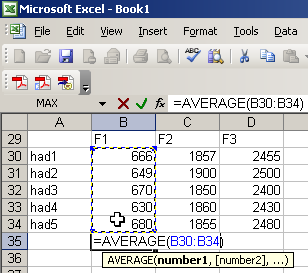
\includegraphics[width=0.8\textwidth]{Excel3}
	\end{center}
\end{figure}


\subsubsection{Plotting}

Once you have the the average formant values, you are ready to plot your data. You should go to \softmenu{Insert} $>$ \softmenu{Chart} (figure~\ref{step1plot}).

\begin{figure}[!tbp]
\caption{\MSExcel{} -- Creating a chart 1}
\label{step1plot}
	\begin{center}
		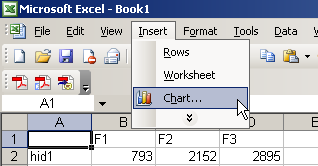
\includegraphics[width=0.8\textwidth]{Excel2}
	\end{center}
\end{figure}

This will open the \softmenu{Chart Wizard} (figure~\ref{step2plot}). Select \softmenu{XY (Scatter)} in the \softmenu{Chart type} field.

\begin{figure}[!tbp]
\caption{\MSExcel{} -- Creating a chart 2}
\label{step2plot}
	\begin{center}
		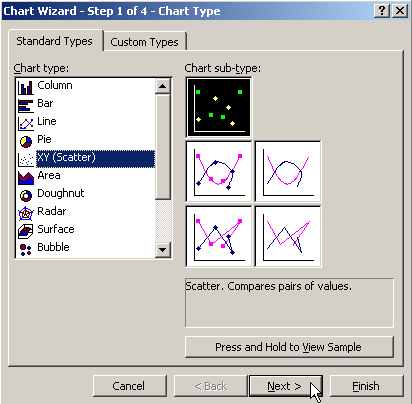
\includegraphics[width=0.8\textwidth]{ExcelPlot1}
	\end{center}
\end{figure}

Now you have to start entering the data. Every word is going to be its own \softmenu{Series}. Figure~\ref{step3plot} shows (schematically) which value goes where; pay attention to the column names, for instance column A is the word name, B is F1, etc. To keep adding words, just click on the \softmenu{Add} button.

\begin{figure}[!tbp]
\caption{\MSExcel{} -- Creating a chart 3}
\label{step3plot}
	\begin{center}
		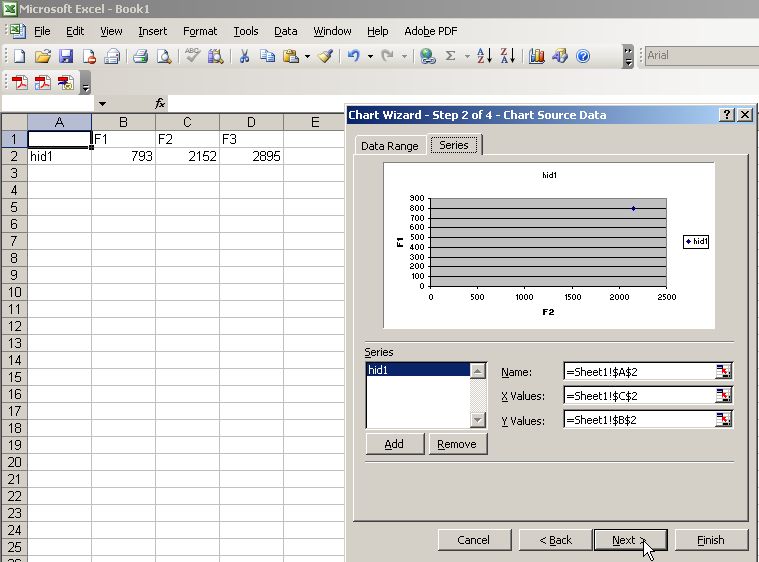
\includegraphics[width=0.8\textwidth]{ExcelPlot3}
	\end{center}
\end{figure}

Once you entered all the series, you can select a name for your graph. The important thing here is to label the axes appropriately. Remember, F1 is supposed to be the y--axis and F2 is supposed to be the x--axis.

\begin{figure}[!tbp]
\caption{\MSExcel{} -- Creating a chart 4}
\label{step3plot}
	\begin{center}
		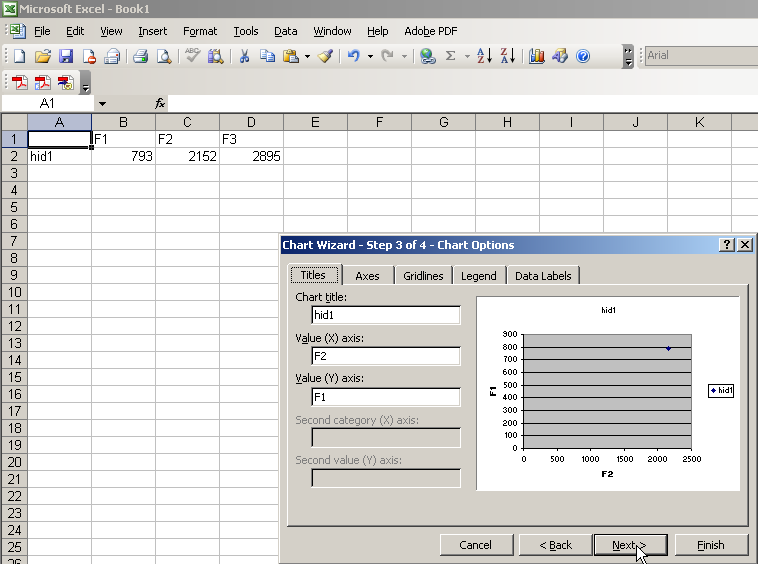
\includegraphics[width=0.8\textwidth]{ExcelPlot4}
	\end{center}
\end{figure}

Finally, once you have the graph ready, you can label the individual points on it. Put the mouse cursor over the point you want to label (figure~\ref{step4plot}) and double click it. This will open the \softmenu{Format Data Series} window. Check the option \softmenu{Series name} (figure~\ref{step5plot})

\begin{figure}[!tbp]
\caption{\MSExcel{} -- Creating a chart 5}
\label{step4plot}
	\begin{center}
		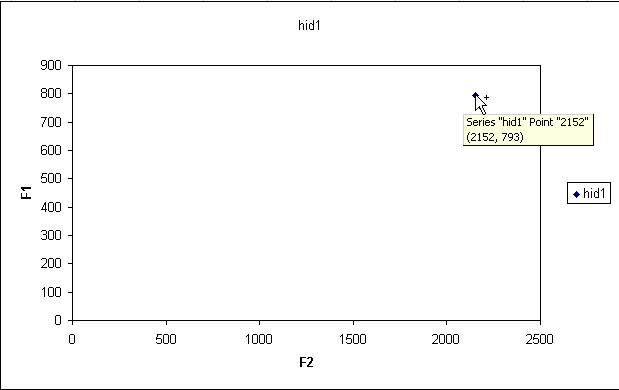
\includegraphics[width=0.8\textwidth]{ExcelPlot5}
	\end{center}
\end{figure}

\begin{figure}[!tbp]
\caption{\MSExcel{} -- Creating a chart 6}
\label{step5plot}
	\begin{center}
		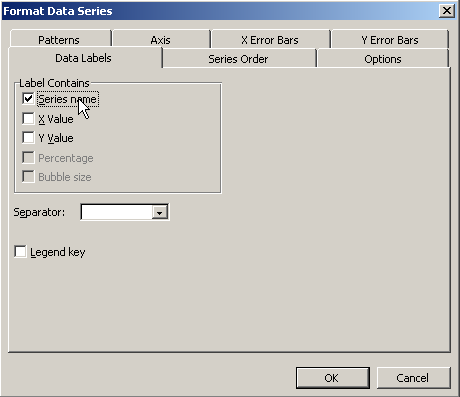
\includegraphics[width=0.8\textwidth]{ExcelPlot6}
	\end{center}
\end{figure}

\subsubsection{Final plot details}

Now that you know how to plot the vowels in a F1 x F2 space, your final graph should look roughly like figure~\ref{step6plot}\footnote{I only plotted three words for simplicity, your graph should have all of them!}

\begin{figure}[!tbp]
\caption{\MSExcel{} -- Creating a chart 7}
\label{step6plot}
	\begin{center}
		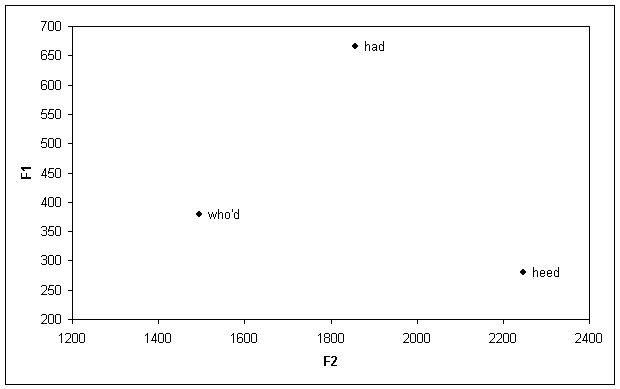
\includegraphics[width=0.8\textwidth]{ExcelPlot7}
	\end{center}
\end{figure}

I'll leave the prettification details of the graph up to you to figure out, since they are not directly relevant to the lab. I won't deduct any points if your graph is not as pretty as it could be, provided the data is accurately portrayed.

However, plotting a graph is not just about being able to see data, but rather being able to see data \emph{in the most informative way} possible. So you should ask yourself certain questions like \emph{Do I need a legend if the points are labeled?}, \emph{Does the range of the scale on the axes make sense?}, and so on and so forth. This will turn out to be important in the future, so keep that in mind.

\paragraph{Write--up:} You should turn in the \MSExcel{} spreadsheet you used to plot your graph and a small write up of your efforts. This report should contain the final plot of the average Formant values of each vowel (all in one plot), a small description of how you got them (did you use Praat's formant track function or did you use the mouse cursor?), the problems you encountered and how you overcame them. Try to motivate your decisions during the process. Most importantly, I'd like you to elaborate on the final plot you obtained: Do you see any pattern or suggestive information on it? If so, what is it and what do you think it means?




\section{Part 2: Finding and measuring acoustic correlates of stop consonants}

In the first part of this lab, you explored the spectrographic representation of different vowels of English. Remember that the driving force behind this was the idea that our "one--to--one mapping" hypothesis about speech perception was worth exploring. In other words, we were exploring the idea that there are pieces of acoustic information that are reliably and univocally associated with segmental representations ($=$vowels and consonants). We started with vowels because in a way they are the ``simplest'' case of speech sounds.

You should think about what the first part of the lab has taught you. As far as vowels are concerned, do you think  that the ``one--to--one'' mapping hypothesis is plausible? Do you think the consonant data we will analyze will be consistent or inconsistent with what we have seen for vowels so far?

By now you already know how to\begin{inparaenum}[(a)]~\item produce a spectrogram, \item identify and extract formant information from a spectrogram, \item plot data in \MSExcel{}\end{inparaenum}. Therefore, the instructions from now on are going to be less detailed.

Now we will proceed to the logical extension of our hypothesis testing, i.e., we will be looking for acoustic correlates of stop consonants in English.The stop consonants we will be looking at are [p b t d k g]. This is not the full inventory of stop consonants in English. Stop consonants receive that name because they are basically a full obstruction of the air flow, produced by either the closure of lips ([p b]), the touch of the tip of the tongue against the alveolar ridge ([t d]) or the touch of the back of the tongue against the velum ([k g]). The place where the flow of air is interrupted is called the \emph{place of articulation} of the consonant.

\subsection{Acoustic correlates of place of articulation in stop consonants}

\subsubsection{Before you start}

As you have probably realized by now, formants can be very visible or hard to see, depending on the vowels and the quality of the recording. In this part of the lab, you will be looking at full syllables. As you are going to realize, the shape of the formants seems to be an important piece of information about consonants. However, you can only analyze their shape if you can see them, right? In some cases, this will require some squinting on your part, especially when F1 and F2 are very close to each other. Don't despair if you feel like you can't see anything. Try a couple of different recordings to see if it improves. If it all seems hopeless, then come see me.

\subsubsection{First step}

First, download \href{http://www.ling.umd.edu/~diogo/courses/ling499a/thebog-thedot-thegod.wav}{this sound file} (a native English speaker uttering \emph{the bog, the dot, the god}\footnote{This is Prof. Bill Idsardi, from the University of Maryland, College Park. The sound file was adapted from some of the files he used for his LING253 class at University of Delaware. I have the feeling that the vowel he uses in \emph{bog} is different than the one he uses in \emph{dot} and \emph{god} (his lab didn't have the same purpose as ours, so it's my fault if that is the case). What do you think? Anyways, we can ignore this for the purposes of our lab; we are not going to analyze his data, but yours.}, open it in \Praat{} (\softmenu{Read} $>$ \softmenu{Read from file\ldots}) and go to the spectrogram view. Can you spot any differences between the consonants? This spectrogram should give you an idea of what you will be looking at from now on. Even though your recordings are probably going to be of lower quality than this one, this spectrogram should be a good reference for you.

\subsubsection{Bab Dad Gag}

There are two files containing the three syllables: \emph{bab dad gag} (ie, two different speakers). Open them in \Praat{} and choose one on your \softmenu{Objects} list. Open the \softmenu{View \& Edit} window. It should look like figure~\ref{step1triplet}:

\begin{figure}[!tbp]
\caption{\Praat{} -- Spectrograms of \emph{Bab Dad Gag}}
\label{step1triplet}
	\begin{center}
		\includegraphics[width=0.8\textwidth]{triplet-badaga1}
	\end{center}
\end{figure}

\paragraph{Write--up:} Once you have the triplet optimally displayed in front of you, try to figure out what the differences between the consonants are. Toggle between having the formant tracks on and off. What looks different in each spectrogram? Does the pattern of formants change according to the consonants you uttered? What about the shape of individual formants? You can also change the temporal window of the spectrogram by going to \softmenu{Spectrum} $>$ \softmenu{Spectrogram settings}, and changing \softmenu{Window length (s)} to $0.01$ or $0.015$, as this sometimes helps seeing the formats a little better.

Try to characterize as best as you can the differences you see. Do you think you can, at least tentatively, characterize the different consonants? That is, do you think you can come up with an acoustic definition of what [b] [d] and [g] are?

Remember to save a picture of your display\footnote{If you do not know how to do that, google ``Print Screen'' or ``Screen capture'' together with your operating system name. In case you want to edit (cropping, for instance) the image you captured, you'll have to use an image editor; \href{http://www.irfanview.com/}{IrfanView for Windows} comes to mind as a good simple alternative, \href{http://www.gimp.org/}{GIMP} is a far more complete and complex alternative, and it is cross--platform. In case you notice you are struggling too much with these technicalities, come see me and I'll try to give you some guidance on how to do the print screen and image editing.} and put it in your write up, so I can see what you saw. Once you have a tentative acoustic definition of each consonant, move on to the next comparison.

\subsubsection{Bee Dee G(u)ee}

Do the same thing you did for the triplet \emph{bab, dad, gag}, but for the files containing the following three syllables: \emph{bee}, \emph{dee}, \emph{g(u)ee} (like \emph{key} but with a [g] instead of [k]; not like the interjection \emph{gee}!)

\paragraph{Write--up:} Compare the three syllables. Remeber to try the formant tracks on and off (sometimes they hinder more than they help) and alternating the window length of the spectrogram. What are the differences between the syllables? Are they consistent with the ones you observed for the first triplet? What about the tentative acoustic definitions for the consonants you derived from the previous triplet, do they hold for this new series of syllables?

Remember to save a picture and put it on your write up. Once you have finished this comparison and written it up, move on to the next one.

\subsubsection{Boo Doo Goo}

Do the same thing you did for the previous two triplets, but for the following: \emph{boo}, \emph{doo}, \emph{goo}.

\paragraph{Write--up:} Compare the three syllables. What are the differences between them? Are they consistent with the ones you observed for the first and/or second triplet? What about the tentative acoustic definition for the consonants you derived from the previous triplets, does it hold for this new series of syllables?

Remember to save a picture and put it on your write up. Once you have finished this comparison and written it up, move on to the next one.

\subsubsection{Dee Daa Doo}

Do the same thing you did for the previous three triplets, but now for the following: \emph{dee}, \emph{daa}, \emph{doo}.

\paragraph{Write--up:} Compare the three syllables. Now, instead of having three different consonants and trying to characterize the differences between them, we are looking at the same consonant; therefore you should try to characterize the similarities between the graphs. By now, you have seen spectrograms for different syllables starting with [d]. Have they been consistent so far? Pay close attention at the shape of the formants. What consequences do you think this has for our ``one--to--one mapping'' hypothesis?

Remember to save a picture and put it on your write up. Once you have finished this comparison and written it up, you can move to the final part of the lab.


\section{Part 3: Finding and measuring acoustic correlates of voicing in stop consonants}

So far we have looked at the following consonants: [b], [d] and [g]. However, they constitute only half of the inventory for the English stop consonants. The other half, [p], [t] and [k] are remarkably close in articulatory terms to [b], [d] and [g] --- namely, they respectively share their place of articulation. In fact, the only difference between the two subsets is what phonologists call ``voicing''. The easiest way to grasp what ``voicing'' is is to say [pa] and [ba] with your index and middle fingers on your throat. Notice the difference? Your vocal chords vibrate more when you articulate the latter than when you articulate the former.

Locate and open the sound file \filefmat{thedot\_thetot.wav}, which contains the recording of a native speaker of English\footnote{Again Bill Idsardi, whose help is much appreciated!} uttering \emph{the dot, the tot}.

Open this file on \Praat{} (\softmenu{Read} $>$ \softmenu{Read from file\ldots}) and get the \softmenu{View \& Edit} window opened. It should look like figure~\ref{step1VOT}.

\begin{figure}[!tbp]
\caption{\Praat{} -- Spectrogram of \emph{the dot, the tot}}
\label{step1VOT}
	\begin{center}
		\includegraphics[width=0.8\textwidth]{VOT-thedotthetot1}
	\end{center}
\end{figure}

\paragraph{Write--up:} Can you see the difference between the voiced (\emph{dot}) and unvoiced (\emph{tot}) consonants? What is it? (Tip: you should look at the waveform as well, since it is also informative).

Once you have figured this one out and written it up, move on.

\paragraph{Write--up:} The difference you observed between the two consonants ([d] and [t]) is called the ``burst'', and it is the flow of air following the release of the stop. Notice how it has energy spread over a wide range of frequencies (the big relatively uniform grayish area before the vowel), and how it is especially salient for [t]; [d] has barely any visible burst on the display. The time between the onset of the burst (i.e., the stop release) and the onset of voicing (in this case, the vowel) receives the name of Voice Onset Time, or simply VOT. Since this seems to be the acoustic cue that sets voiced and unvoiced stop consonants apart, we are going to be measuring it.

Your task now is to open the files containing the recordings of a different native speaker of American English saying the two words (\emph{the dot, the tot}) and measure the VOT of both consonants.

Here's how you do it. First, zoom in in the \emph{the tot} utterance, as shown in figure~\ref{step2VOT}. Now, try to find and select the chunk of time between the onset of the burst and the onset of the vowel, as shown in figure~\ref{step3VOT}. 
\begin{figure}[!tbp]
\caption{\Praat{} -- Spectrogram of \emph{the dot, the tot} -- zooming in}
\label{step2VOT}
	\begin{center}
		\includegraphics[width=0.8\textwidth]{VOT-thedotthetot-zoom}
	\end{center}
\end{figure}

\begin{figure}[!tbp]
\caption{\Praat{} -- Spectrogram of \emph{the dot, the tot} -- Measuring the VOT of [t]}
\label{step3VOT}
	\begin{center}
		\includegraphics[width=0.8\textwidth]{VOT-thedotthetot-measuring-unvoiced}
	\end{center}
\end{figure}

Once you are confident in your selection, go to \softmenu{Query} $>$ \softmenu{Get selection length}, and copy and paste the value you get into a spreadsheet, as shown in figure~\ref{step4VOT} --- notice the little trick to transform the measurements from seconds to miliseconds.

\begin{figure}[!tbp]
\caption{\MSExcel{} -- Saving your measurements}
\label{step4VOT}
	\begin{center}
		\includegraphics[width=0.8\textwidth]{VOT-thedotthetot-Excel01}
	\end{center}
\end{figure}

Now you should try to measure the VOT of [d]. Unzoom from where you are (\softmenu{View} $>$ \softmenu{Show all}) and zoom in on the first utterance. As you can see in figure~\ref{step5VOT}, the VOT is much smaller than the one for [t]. In fact, it is very possible you will need to zoom in some more in your own recordings to see the burst at all, since the quality of the recording will probably not be as good. Once you are satisfied with your selection, get the values into the spreadsheet.

\begin{figure}[!tbp]
\caption{\Praat{} -- Spectrogram of \emph{the dot, the tot} -- Measuring the VOT of [d]}
\label{step5VOT}
	\begin{center}
		\includegraphics[width=0.8\textwidth]{VOT-thedotthetot-measuring-voiced}
	\end{center}
\end{figure}
 
Try to get the values of the 15 repetitions files. By the end, your spreadsheet should look something like figure~\ref{step6VOT}.

\begin{figure}[!tbp]
\caption{\MSExcel{} -- What your spreadsheet should look like}
\label{step6VOT}
	\begin{center}
		\includegraphics[width=0.8\textwidth]{VOT-thedotthetot-Excel03}
	\end{center}
\end{figure}

\paragraph{Write--up:} Notice the time--bins (0--10, 10--20, \dots{}, 90--100) on the bottom of the spreadsheet, with two empty columns, one under [t] and one under [d]. Your task now is to populate these columns with the counts of how many observations you had in each time--bin. For instance, if you had two [t] VOTs falling into the bin 60--70ms, then you should input ``2'' on the column ``[t]'' next to the bin ``60--70''. Once you are done, you should plot a bar graph of the data you collected, with the time--bins as the x--axis and the counts on the y--axis, as shown in figure~\ref{step7VOT}. What can you conclude from your graph? Does VOT constitute a good acoustic cue to differentiate voiced and unvoiced stops? What are the consequences for our ``one--to--one mapping'' hypothesis?

\begin{figure}[!tbp]
\caption{\MSExcel{} -- Plotting the VOT bar graph}
\label{step7VOT}
	\begin{center}
		\includegraphics[width=0.8\textwidth]{VOT-thedotthetot-Excel04}
	\end{center}
\end{figure}
 
\section{What you need to write up}

All the parts marked as \emph{Write--up} in the instructions above should be incorporated in your lab write--up, together with the plots they require. Try to articulate your impressions and results the best you can, in full coherent sentences (no bullets, please).

As a conclusion to your write--up, try to evaluate where our ``one--to--one mapping'' hypothesis stand. Were any of your data consistent with it? If so, which and how? Were any data inconsistent with it? If so, which and how? After this exercise, what is your feeling about our initial hypothesis? Is it still tenable? Plausible? Do you think you need more data before you commit either way? If so, why and what kind of data would that be?

\section{What you need to hand in}

You should send me your write--up and your Excel spreadsheet(s) by e-mail.

\section{Deadline}

This lab is due by \emph{e--mail} on \emph{Thursday, March 21st, by 11 pm}.


\end{document}